
\chapter*{Prólogo}
\section{Sobre esta materia}

\begin{itemize}
 \item  \href{https://docs.google.com/viewer?a=v&pid=sites&srcid=ZGVmYXVsdGRvbWFpbnxlY3VhY2lvbmVzZGlmZXJlbmNpYWxldW5yY3xneDoyZjE0YzJmMDcyODc0ZGQ3}{Programa analítico.}
 \item  \href{https://sites.google.com/site/ecuacionesdiferencialeunrc/ecuaciones-diferenciales-unrc}{Página web} de la materia
 \item  Vamos a hacer uso intensivo de paquetes de matemática basados en \href{https://www.python.org/}{Python}, por ejemplo \href{http://www.scipy.org/}{SciPy},  \href{http://www.scipy.org/}{SymPy} y \href{http://www.sagemath.org/}{SAGE}.
 \item  Requeriremos muchos contenidos de la asignatura Física.
 \item  \begin{tabular}{m{4cm} m{2cm} m{2cm}} Bibliografía principal & 
\includegraphics[scale=0.05]{imagenes/Tapa_Simmons.jpg} &    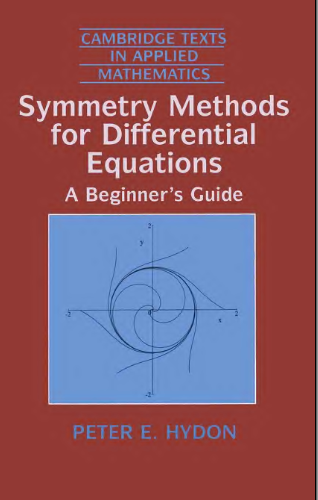
\includegraphics[scale=0.13]{imagenes/tapa_hydon.png}          \end{tabular}

\end{itemize}

